%%%%%%%%%%%%%%%%%%%%%%%%%%%%%%%%%%%%%%%%%
% Beamer Presentation - LaTeX Template
% Version 2.0 (March 8, 2022)
% Original Template: https://www.LaTeXTemplates.com
% Author: Vel (vel@latextemplates.com)
% License: CC BY-NC-SA 4.0

% Este modelo de apresentação foi 
% criado a partir do modelo de Giovanni Spadaro.
% Disponível em: https://github.com/Giovo17/presentation-template-unict-lm-data
%
% Adaptado por Lucas Amaral Taylor para criar uma versão especial 
% para os alunos de Matemática e Estatística da USP (IME-USP).
% Disponível em: https://github.com/lucasamtaylor01/IME-template
%%%%%%%%%%%%%%%%%%%%%%%%%%%%%%%%%%%%%%%%%

%----------------------------------------------------------------------------------------
% CLASSE DO DOCUMENTO E CONFIGURAÇÕES BÁSICAS
%----------------------------------------------------------------------------------------
\documentclass[
    11pt,               % Tamanho padrão da fonte
    % t,                % Alinhar verticalmente ao topo
    %aspectratio=169,   % Definir proporção 16:9
]{beamer}
\graphicspath{{img/}}         % Define o diretório das imagens

%----------------------------------------------------------------------------------------
% PACOTES NECESSÁRIOS
%----------------------------------------------------------------------------------------
\usepackage{
    booktabs,     % Melhora a aparência das linhas em tabelas
    palatino,     % Define Palatino como fonte principal
    subcaption    % Suporte para subfiguras
}
\usepackage[default]{opensans}  % Define Open Sans como fonte secundária
%----------------------------------------------------------------------------------------
%	PACOTES E CONFIGURAÇÕES PARA CÓDIGO
%----------------------------------------------------------------------------------------
% Pacotes necessários para formatação de código
\usepackage[utf8]{inputenc}
\usepackage{listings}
\usepackage{xcolor}

% Cores para syntax highlighting (VSCode Light Theme)
\definecolor{vscBackground}{RGB}{255,255,255}    % Fundo branco
\definecolor{vscKeyword}{RGB}{175,0,219}         % Roxo para palavras-chave
\definecolor{vscString}{RGB}{163,21,21}          % Vermelho para strings
\definecolor{vscComment}{RGB}{0,128,0}           % Verde para comentários
\definecolor{vscFunction}{RGB}{121,94,38}        % Marrom para funções
\definecolor{vscNumber}{RGB}{9,134,88}           % Verde escuro para números
\definecolor{vscOperator}{RGB}{175,0,219}        % Roxo para operadores
\definecolor{vscText}{RGB}{0,0,0}                % Texto preto
\definecolor{vscLineNr}{RGB}{128,128,128}        % Cinza para números de linha

% Configuração geral do listings para UTF-8
\lstset{
    inputencoding=utf8,
    extendedchars=true,
    literate=%
        {á}{{\'a}}1 {é}{{\'e}}1 {í}{{\'i}}1 {ó}{{\'o}}1 {ú}{{\'u}}1
        {Á}{{\'A}}1 {É}{{\'E}}1 {Í}{{\'I}}1 {Ó}{{\'O}}1 {Ú}{{\'U}}1
        {à}{{\`a}}1 {è}{{\`e}}1 {ì}{{\`i}}1 {ò}{{\`o}}1 {ù}{{\`u}}1
        {À}{{\`A}}1 {È}{{\'E}}1 {Ì}{{\`I}}1 {Ò}{{\`O}}1 {Ù}{{\`U}}1
        {ã}{{\~a}}1 {ẽ}{{\~e}}1 {ĩ}{{\~i}}1 {õ}{{\~o}}1 {ũ}{{\~u}}1
        {Ã}{{\~A}}1 {Ẽ}{{\~E}}1 {Ĩ}{{\~I}}1 {Õ}{{\~O}}1 {Ũ}{{\~U}}1
        {â}{{\^a}}1 {ê}{{\^e}}1 {î}{{\^i}}1 {ô}{{\^o}}1 {û}{{\^u}}1
        {Â}{{\^A}}1 {Ê}{{\^E}}1 {Î}{{\^I}}1 {Ô}{{\^O}}1 {Û}{{\^U}}1
        {ç}{{\c c}}1 {Ç}{{\c C}}1
        {º}{{\textordmasculine}}1
        {ª}{{\textordfeminine}}1
}

% Configurações base comum para todas as linguagens
\lstdefinestyle{baseStyle}{
    backgroundcolor=\color{vscBackground},
    basicstyle=\ttfamily\small\color{vscText},
    breakatwhitespace=false,
    breaklines=true,
    captionpos=b,
    keepspaces=true,
    numbers=left,
    numbersep=5pt,
    showspaces=false,
    showstringspaces=false,
    showtabs=false,
    tabsize=4,
    frame=single,
    framerule=0.8pt,
    rulecolor=\color{gray!20},
    numberstyle=\tiny\color{vscLineNr},
    keywordstyle=\color{vscKeyword},
    commentstyle=\color{vscComment}\itshape,
    stringstyle=\color{vscString},
    emphstyle=\color{vscFunction},
    columns=flexible,
    basewidth={0.5em,0.45em},
    inputencoding=utf8,
    extendedchars=true
}

%----------------------------------------------------------------------------------------
% Python
%----------------------------------------------------------------------------------------
\lstdefinestyle{pythonStyle}{
    style=baseStyle,
    language=Python,
    morekeywords={self,None,True,False,import,from,as,def,class,return,yield,
                  for,while,if,else,elif,try,except,finally,with,lambda,
                  async,await,break,continue,global,nonlocal,pass,raise},
    morekeywords=[2]{print,len,range,type,int,str,float,list,dict,set,
                     tuple,max,min,sum,sorted,enumerate,zip,map,filter,
                     any,all,abs,round,pow,divmod},
    keywordstyle=[2]\color{vscFunction},
    sensitive=true
}

\lstnewenvironment{python}[1][]{\lstset{style=pythonStyle, #1}}{}
\newcommand{\pyinline}[1]{\lstinline[style=pythonStyle]!#1!}
\newcommand{\inputpython}[2][]{\lstinputlisting[style=pythonStyle,#1]{#2}}

%----------------------------------------------------------------------------------------
% C Language
%----------------------------------------------------------------------------------------
\lstdefinestyle{cStyle}{
    style=baseStyle,
    language=C,
    morekeywords={include,define,void,int,char,float,double,long,unsigned,
                  struct,union,enum,typedef,const,static,extern,register,
                  auto,volatile,sizeof,return,if,else,for,while,do,switch,
                  case,break,continue,default,goto},
    morekeywords=[2]{printf,scanf,malloc,free,calloc,realloc,fopen,fclose,
                     fprintf,fscanf,strcpy,strlen,strcat},
    keywordstyle=[2]\color{vscFunction},
    sensitive=true
}

\lstnewenvironment{clang}[1][]{\lstset{style=cStyle, #1}}{}
\newcommand{\clinline}[1]{\lstinline[style=cStyle]!#1!}
\newcommand{\inputclang}[2][]{\lstinputlisting[style=cStyle,#1]{#2}}

%----------------------------------------------------------------------------------------
% C++
%----------------------------------------------------------------------------------------
\lstdefinestyle{cppStyle}{
    style=baseStyle,
    language=C++,
    morekeywords={class,private,protected,public,template,typename,namespace,
                  using,new,delete,this,friend,virtual,override,final,explicit,
                  mutable,constexpr,nullptr,noexcept,static_cast,dynamic_cast,
                  const_cast},
    morekeywords=[2]{cout,cin,endl,vector,string,map,set,queue,stack,pair,
                     begin,end,push_back,pop_back,emplace_back,size,empty},
    keywordstyle=[2]\color{vscFunction},
    sensitive=true
}

\lstnewenvironment{cpp}[1][]{\lstset{style=cppStyle, #1}}{}
\newcommand{\cppinline}[1]{\lstinline[style=cppStyle]!#1!}
\newcommand{\inputcpp}[2][]{\lstinputlisting[style=cppStyle,#1]{#2}}

%----------------------------------------------------------------------------------------
% R Language
%----------------------------------------------------------------------------------------
\lstdefinestyle{rStyle}{
    style=baseStyle,
    language=R,
    morekeywords={if,else,repeat,while,function,for,in,next,break,TRUE,FALSE,
                  NULL,Inf,NaN,NA,NA_integer_,NA_real_,NA_complex_,NA_character_},
    morekeywords=[2]{library,require,attach,detach,source,setwd,options,
                     data.frame,read.csv,write.csv,list,matrix,array},
    keywordstyle=[2]\color{vscFunction},
    sensitive=true
}

\lstnewenvironment{rlang}[1][]{\lstset{style=rStyle, #1}}{}
\newcommand{\rlinline}[1]{\lstinline[style=rStyle]!#1!}
\newcommand{\inputrlang}[2][]{\lstinputlisting[style=rStyle,#1]{#2}}

%----------------------------------------------------------------------------------------
% Java
%----------------------------------------------------------------------------------------
\lstdefinestyle{javaStyle}{
    style=baseStyle,
    language=Java,
    morekeywords={abstract,assert,boolean,break,byte,case,catch,char,class,
                  const,continue,default,do,double,else,enum,extends,final,
                  finally,float,for,if,implements,import,instanceof,int,
                  interface,long,native,new,package,private,protected,public,
                  return,short,static,strictfp,super,switch,synchronized,this,
                  throw,throws,transient,try,void,volatile,while},
    morekeywords=[2]{String,System,out,println,printStackTrace,ArrayList,
                     HashMap,Arrays,List,Map,Set,Exception,RuntimeException},
    keywordstyle=[2]\color{vscFunction},
    sensitive=true
}

\lstnewenvironment{java}[1][]{\lstset{style=javaStyle, #1}}{}
\newcommand{\javainline}[1]{\lstinline[style=javaStyle]!#1!}
\newcommand{\inputjava}[2][]{\lstinputlisting[style=javaStyle,#1]{#2}}       % Importa configurações para highlight de código

%----------------------------------------------------------------------------------------
% CONFIGURAÇÃO DO TEMA
%----------------------------------------------------------------------------------------
% Tema Base
\usetheme{Boadilla}                            % Define o tema principal
\useinnertheme{circles}                        % Tema interno com círculos
\useoutertheme[subsection = false]{miniframes} % Tema externo com miniframes
\setbeamertemplate{navigation symbols}{}       % Remove símbolos de navegação

% Cores Personalizadas
\definecolor{primaryColor}{RGB}{20,45,105}     % Cor primária - azul escuro
\definecolor{secondaryColor}{RGB}{0,100,160}   % Cor secundária - azul médio

% Configurações de Cores
\setbeamercolor{structure}{fg=primaryColor}
\setbeamercolor{palette primary}{bg=primaryColor, fg=white}
\setbeamercolor{palette secondary}{bg=secondaryColor, fg=white}
\setbeamercolor{title}{bg=primaryColor, fg=white}

% Cores do Cabeçalho e Rodapé
\setbeamercolor{headline}{bg=secondaryColor, fg=white}
\setbeamercolor{section in head/foot}{bg=primaryColor, fg=white}
\setbeamercolor{subsection in head/foot}{bg=secondaryColor, fg=white}
\setbeamercolor{author in head/foot}{bg=primaryColor, fg=white}
\setbeamercolor{title in head/foot}{bg=secondaryColor, fg=white}
\setbeamercolor{date in head/foot}{bg=primaryColor, fg=white}
\setbeamercolor{page number in head/foot}{bg=primaryColor, fg=white}

%----------------------------------------------------------------------------------------
% BIBLIOGRAFIA
%----------------------------------------------------------------------------------------
% \usepackage{biblatex}
% \addbibresource{bibliografia.bib}

%----------------------------------------------------------------------------------------
% INFORMAÇÕES DA APRESENTAÇÃO
%----------------------------------------------------------------------------------------
\title[Análise de Métricas em OET]{Comparativo de Métricas Intrínsecas para Avaliação de Modelos em Open-Ended Tasks}          % [Versão curta]{Versão completa}
\author[Eduardo D. Faé]{Eduardo Dalmás Faé} % [Versão curta]{Nome completo}
\institute[INF-UFRGS]{Instituto de Informática - UFRGS}
\date[2025]{Julho / 2025}

%----------------------------------------------------------------------------------------
% INÍCIO DO DOCUMENTO
%----------------------------------------------------------------------------------------
\begin{document}

% Slide de título com logo
\begin{frame}[plain,t]
    \begin{figure}
        
\includegraphics[height=0.2\textheight]{UFRGS-logo.png}
        \hspace{100px}
        
\includegraphics[height=0.2\textheight]{INF-logo.png}
    \end{figure}
    \titlepage
\end{frame}

% Sumário
\begin{frame}
    \frametitle{Estrutura da apresentação}
    \tableofcontents
\end{frame}

% Inclusão das seções
\section{Introdução} % Seções são adicionadas para organizar sua apresentação em blocos discretos, todas as seções e subseções são automaticamente exibidas no índice como uma visão geral da apresentação, mas NÃO são exibidas como slides separados.

%----------------------------------------------------------------------------------------

% \begin{frame}
% 	\frametitle{Problema}
% 	\begin{itemize}[<+(1)->]
% 		\item Avaliar o desempenho de modelos na resolução de Open-Ended Tasks é difícil.
% 		\item Novas métricas automatizadas seguem sendo desenvolvidas.
% 		\item Qual a melhor métrica para cada situação?
% 		\only<5>{
% 			\item Como as métricas se correlacionam com avaliações humanas?
% 		}
% 		\only<6>{
% 			\item \textbf{Como as métricas se correlacionam com avaliações humanas?}
% 		}
% 	\end{itemize}
% \end{frame}

%----------------------------------------------------------------------------------------

% \begin{frame}
% 	\frametitle{Objetivo}
% 	Mensurar a correlação entre diferentes métricas de avaliação automatizadas e 
% 	a forma de avaliação humana no âmbito de open-ended tasks em português.
% \end{frame}

%----------------------------------------------------------------------------------------

% \begin{frame}
% 	\only<1>{
% 		\frametitle{Processamento de Linguagem Natural}
% 	}
% 	\only<2>{
% 		\frametitle{Processamento de Linguagem Natural (PLN)}
% 	}
% 	\only<3->{
% 		\frametitle{PLN}
% 	}
% 	\only<3-8>{
% 		\begin{columns}
% 			\column{0.5\linewidth}
% 				Permitir ao modelo:
% 				\begin{itemize}[<+(3)-8>]
% 					\item Compreender
% 					\item Interpretar
% 					\item Analisar
% 					\item Reproduzir
% 				\end{itemize}
% 			\column{0.5\linewidth}
% 				\only<8>{
% 					\begin{figure}
% 						
\includegraphics[width=\textwidth]{linguagem-natural.jpg}
% 						\caption{Linguagem Natural}
% 					\end{figure}
% 				}
% 		\end{columns}
% 	}
% 	\only<9>{
% 		\begin{figure}
% 			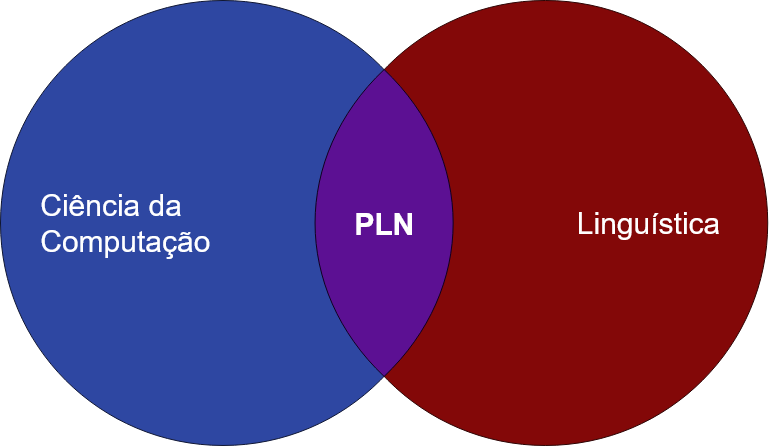
\includegraphics[width=0.8\textwidth]{PLN-AREA.png}
% 		\end{figure}
% 	}
% 	\only<10>{
% 		\begin{figure}
% 			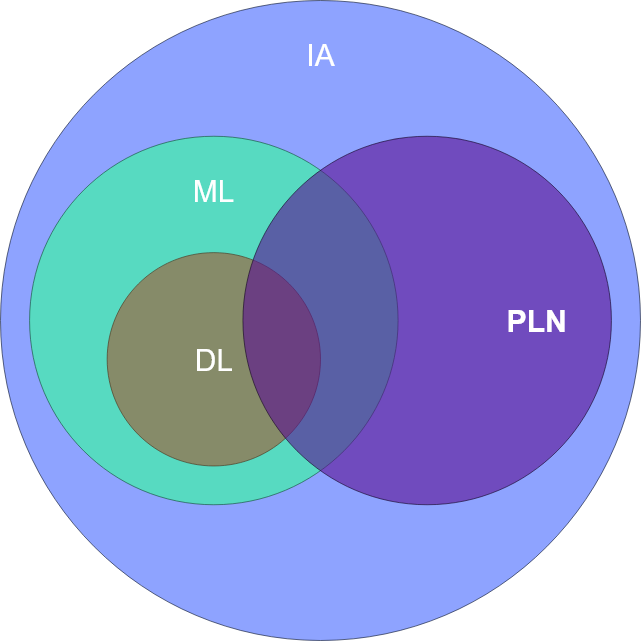
\includegraphics[height=0.8\textheight]{PLN-IA.png}
% 		\end{figure}
% 	}
% 	\only<11>{
% 		Desde a concepção dos primeiros computadores, já se sonhava com a ideia 
% 		de que os mesmos conseguissem compreender a linguagem humana.
% 	}
% \end{frame}

% %----------------------------------------------------------------------------------------

% \begin{frame}
% 	\only<1-4>{
% 		\frametitle{Teste de Turing}
% 	}
% 	\only<5->{
% 		\frametitle{Problemas do Teste}
% 	}
% 	\only<1-3>{
% 		\begin{columns}
% 			\column{0.5\linewidth}
% 				\begin{itemize}[<+(1)-3>]
% 					\item Proposto em 1950.
% 					\item \textbf{Máquina} consegue emular comportamento \textbf{humano}.
% 				\end{itemize}
% 			\column{0.5\linewidth}
% 				\begin{figure}
% 					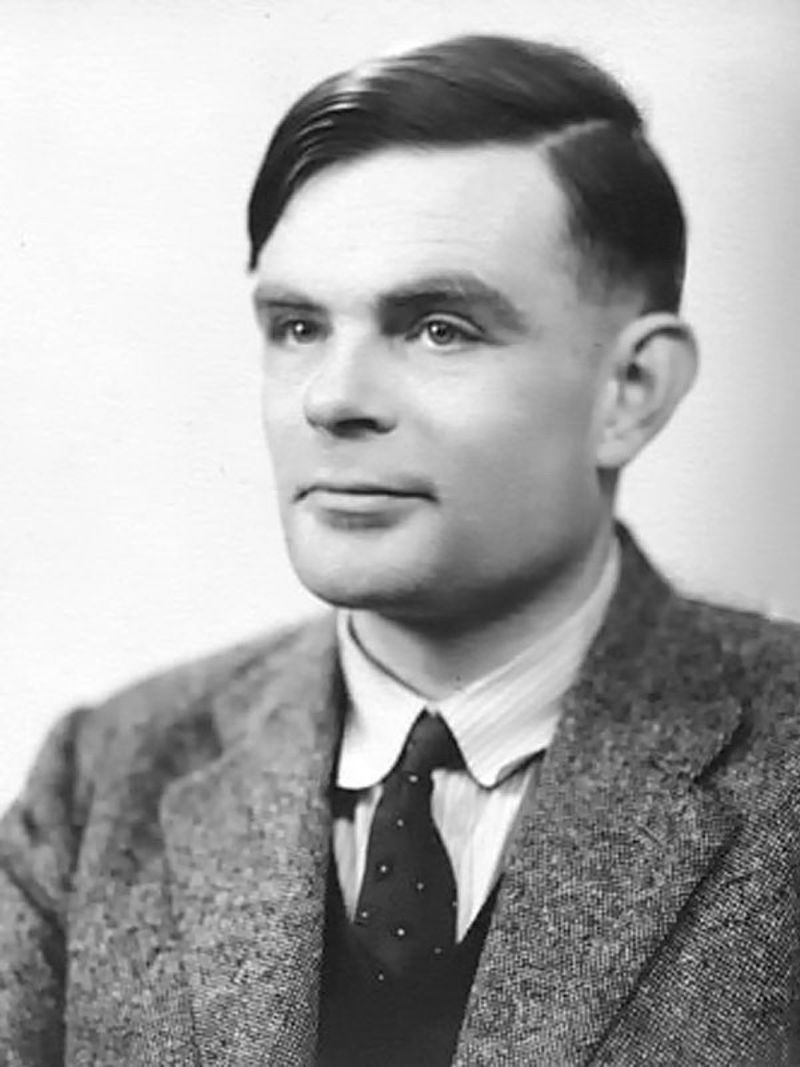
\includegraphics[height=0.6\textheight]{Turing.jpg}
% 					\caption{Alan Turing}
% 				\end{figure}
% 		\end{columns}
% 	}
% 	\only<4>{
% 		\begin{figure}
% 			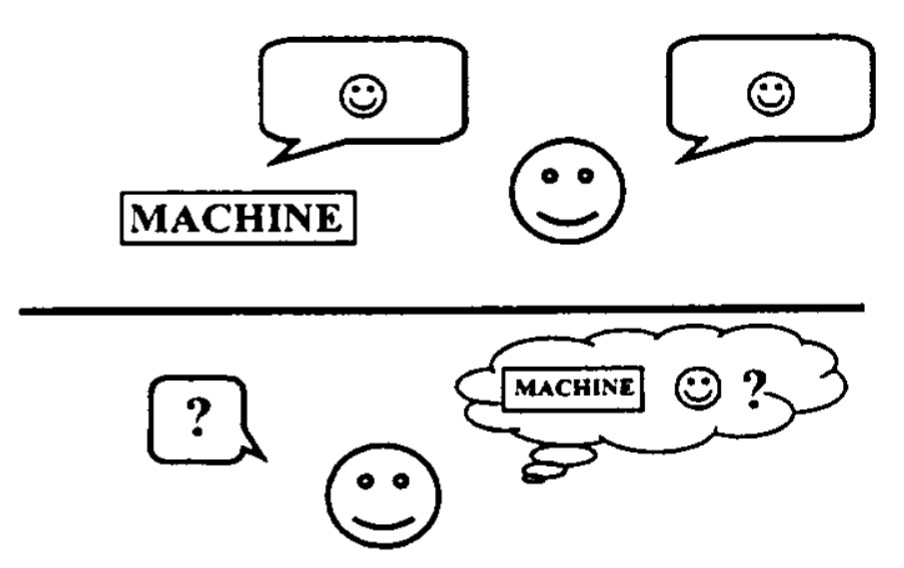
\includegraphics[width=0.8\textwidth]{Turing Test.jpg}
% 			% \caption{Fonte: \citet{pinar2000turing}.}
% 		\end{figure}
% 	}
% 	\only<5->{
% 		\begin{itemize}[<+(5)->]
% 			\item Fácil Manipulação.
% 			\item Falta de Autoconsciência.
% 			\only<8>{
% 				\item Imitação vs Compreensão.
% 			}
% 			\only<9>{
% 				\item \textbf{Imitação vs Compreensão.}
% 			}
% 		\end{itemize}
% 	}
% \end{frame}

% %----------------------------------------------------------------------------------------

% \begin{frame}
% 	\frametitle{Argumento do Quarto Chinês}
% 	\only<1-3>{
% 		\begin{columns}
% 			\column{0.5\linewidth}
% 				\begin{itemize}[<+(1)-3>]
% 					\item Proposto em 1980.
% 					\item Questiona pressuposições do Teste de Turing.
% 				\end{itemize}
% 			\column{0.5\linewidth}
% 				\begin{figure}
% 					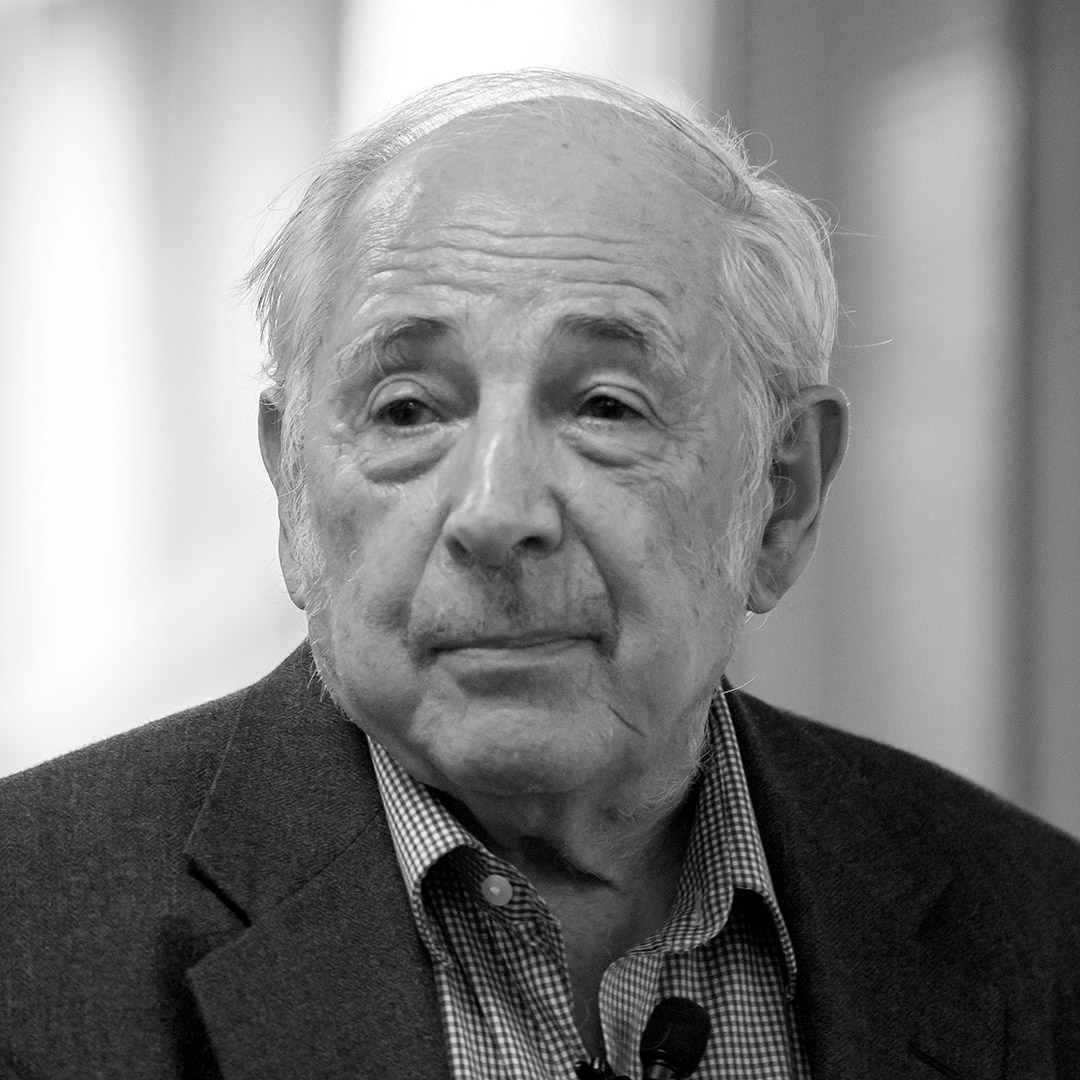
\includegraphics[height=0.6\textheight]{John_Searle.jpg}
% 					\caption{John R. Searle}
% 				\end{figure}
% 		\end{columns}
% 	}
% 	\only<4>{
% 		\begin{figure}
% 			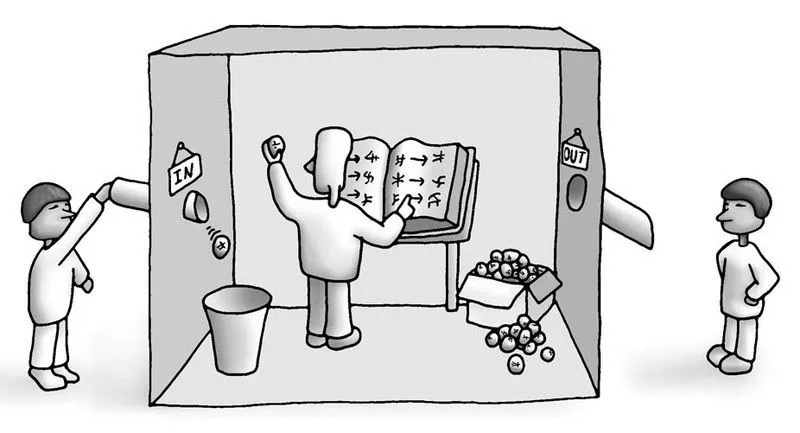
\includegraphics[width=0.8\textwidth]{o-quarto-chines.jpg}
% 			% \caption{Fonte: \citet{pinar2000turing}.}
% 		\end{figure}
% 	}
% 	\only<5>{
% 		Esse argumento evidencia a dificuldade presente em avaliar a real 
% 		capacidade de uma máquina executando tarefas humanas.
% 	}
% \end{frame}

%----------------------------------------------------------------------------------------

% \begin{frame}
% 	\frametitle{Large Language Models}
% \end{frame}

%----------------------------------------------------------------------------------------

\begin{frame}
	\frametitle{Open-Ended Tasks}
	\only<1-5>{
		\begin{itemize}[<+(1)->]
			\item Permitem diferentes interpretações e soluções. 
			\item Primariamente subjetivas.
			\item Comumente presente em áreas que exigem criatividade e pensamento crítico.
			\item Extremamente comuns em PLN.
		\end{itemize}
	}
	\only<6>{
		\frametitle{Exemplos}
		\begin{columns}
			\column{0.5\linewidth}
				\begin{figure}
					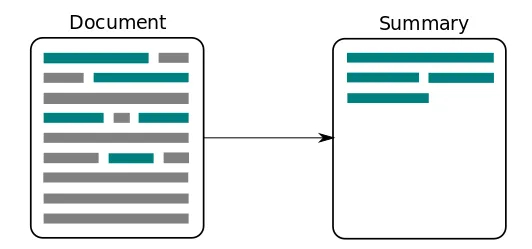
\includegraphics[width=0.8\textwidth]{summ.png}
					\caption{Sumarização}
				\end{figure}
			\column{0.5\linewidth}
				\begin{figure}
					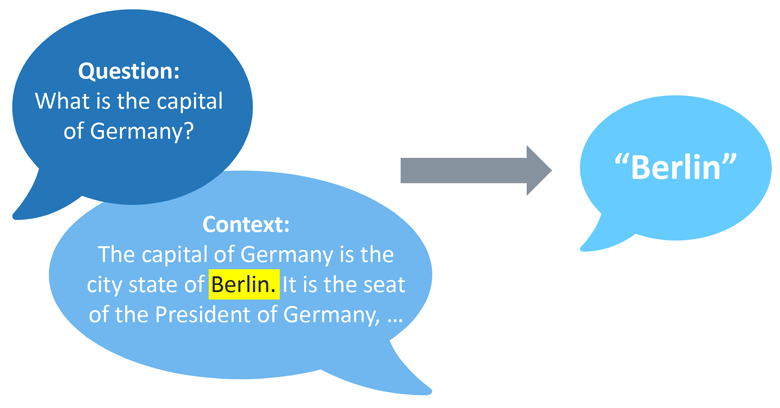
\includegraphics[width=0.8\textwidth]{qamainimage.png}
					\caption{Question-Answering}
				\end{figure}
		\end{columns}
	}
\end{frame}

%----------------------------------------------------------------------------------------

\begin{frame}
	\only<1>{
		\frametitle{Avaliação Intínseca x Extrínseca}
		\begin{figure}
			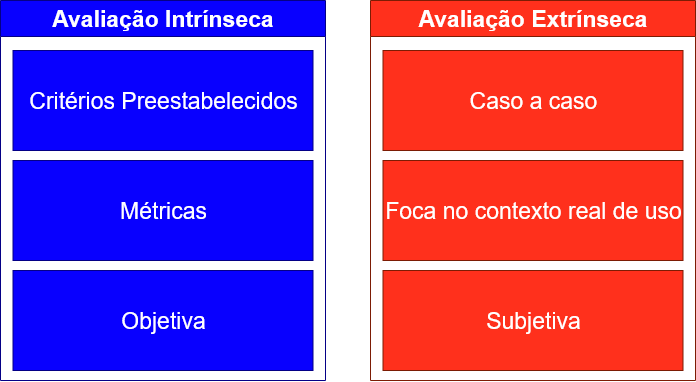
\includegraphics[width=0.8\textwidth]{TCC-Extrinsic-Intrinsic.png}
		\end{figure}
	}
	\only<3->{
		\frametitle{Avaliação de Open-Ended Tasks}
	}
	\only<2>{
		\frametitle{Avaliação Intínseca}
		\begin{figure}
			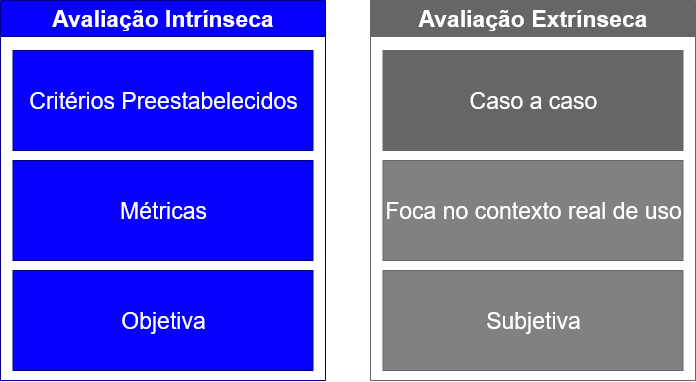
\includegraphics[width=0.8\textwidth]{TCC-Extrinsic-Intrinsic-Chosen.png}
		\end{figure}
	}
	\only<3>{
		\begin{figure}
			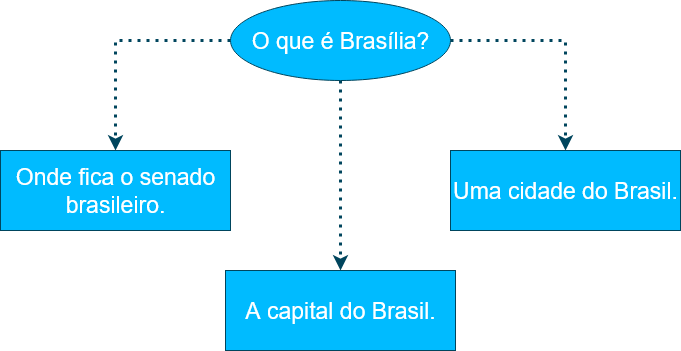
\includegraphics[width=0.8\textwidth]{TCC-qa-dificulty-example.png}
		\end{figure}
	}
	\only<4>{
		\begin{figure}
			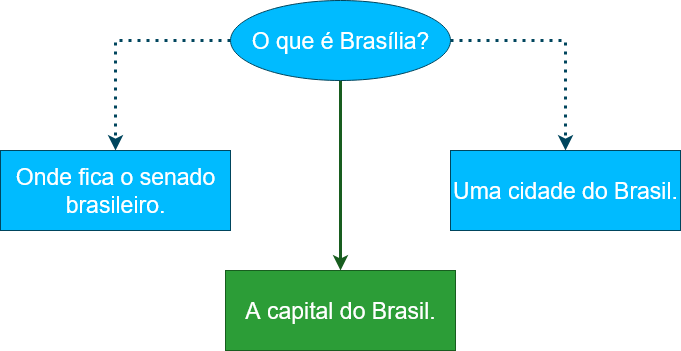
\includegraphics[width=0.8\textwidth]{TCC-qa-dificulty-example-resposta_esperada.png}
		\end{figure}
	}
	\only<5>{
		\begin{figure}
			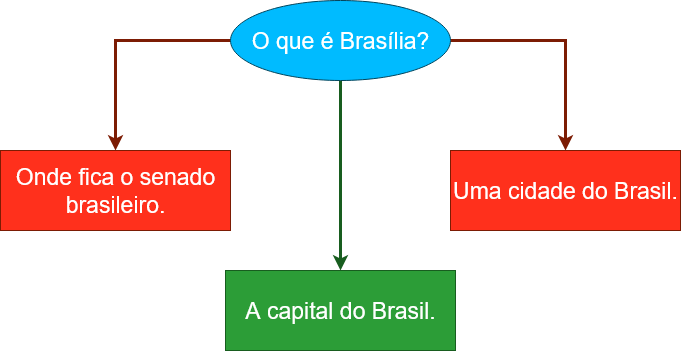
\includegraphics[width=0.8\textwidth]{TCC-qa-dificulty-example-problem.png}
		\end{figure}
	}
	\only<6>{
		\begin{figure}
			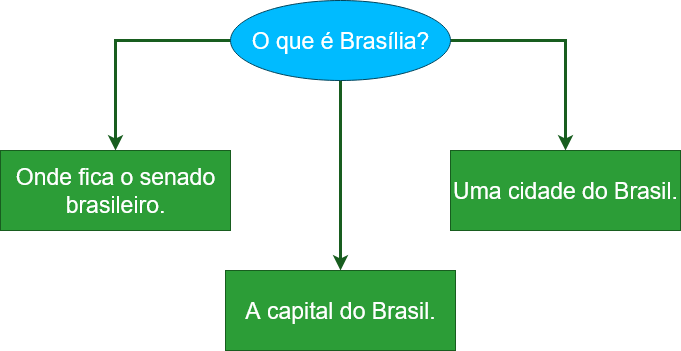
\includegraphics[width=0.8\textwidth]{TCC-qa-dificulty-example-esperado.png}
		\end{figure}
	}
	% \only<6->{
	% 	\begin{center}
	% 		Um cachorro foi ao parque se divertir, lá encontrou um gato. Após 
	% 		encontrá-lo o cachorro passou a tarde correndo atrás do mesmo.
	% 	\end{center}
	% 	\begin{columns}
	% 		\column{0.5\linewidth}
	% 		\begin{center}
	% 			O cachorro foi ao parque e brincou com o gato.
	% 		\end{center}
	% 		\column{0.5\linewidth}
	% 		\begin{center}
	% 			O cachorro passou a tarde correndo atrás do gato no parque.
	% 		\end{center}
	% 	\end{columns}
	% }
\end{frame}

%----------------------------------------------------------------------------------------

\begin{frame}
	\frametitle{Métricas Baseadas em N-Gramas}
	\only<2>{
		\begin{figure}
			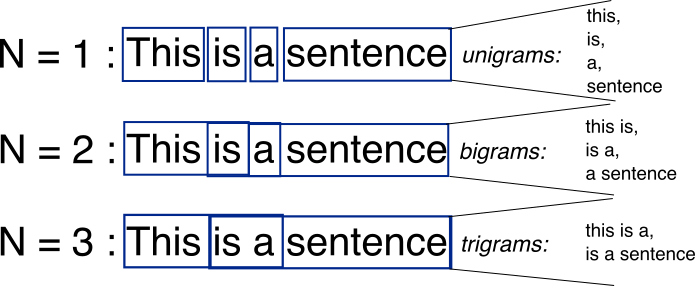
\includegraphics[width=0.8\textwidth]{n-grams.png}
		\end{figure}
	}
	\only<3>{
		\begin{figure}
			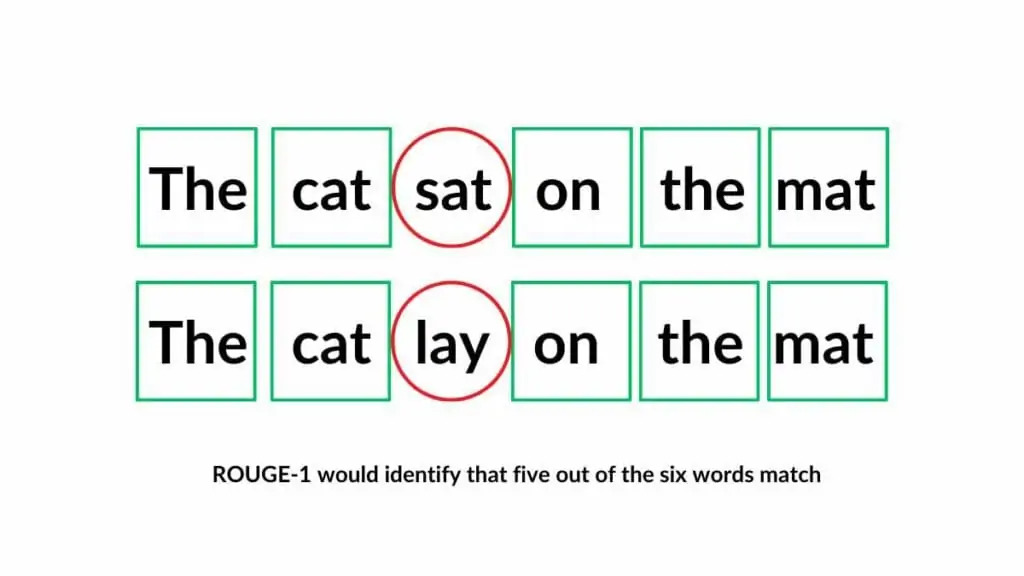
\includegraphics[width=0.8\textwidth]{ROUGE-1-example-1024x576.jpg}
		\end{figure}
	}
	\only<4>{
		\frametitle{Métricas Mais Populares}
		\begin{itemize}
			\item BLEU
			\item ROUGE
			\item METEOR
		\end{itemize}
	}
	\only<5-7>{
		\frametitle{Problemas desse tipo de métrica}
		\begin{itemize}[<+(5)->]
			\item Não capturam significado semântico.
			\item Dificuldade em reconhecer sinônimos.
		\end{itemize}
	}
	\only<8>{
		\frametitle{Problemas desse tipo de métrica}
		\begin{figure}
			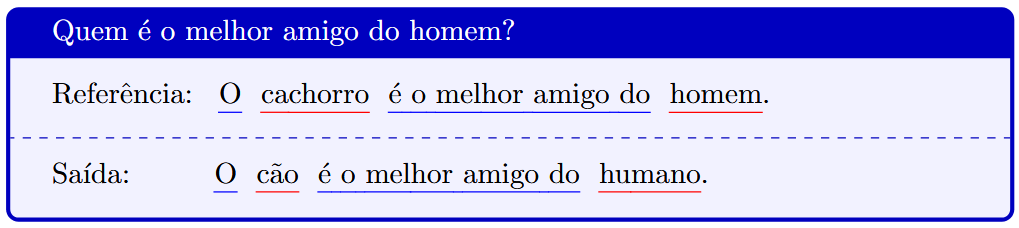
\includegraphics[width=0.9\textwidth]{sinonimos-problema.png}
		\end{figure}
	}
\end{frame}

%----------------------------------------------------------------------------------------

\begin{frame}
	\frametitle{Métricas Baseadas em PLMs}
	\only<2>{
		\begin{columns}
			\column{0.5\textwidth}
			\begin{figure}
				
\includegraphics[height=0.6\textheight]{Bert_smile.png}
				\caption{BERT (Devlin et al., 2019)}
			\end{figure}
			\column{0.5\textwidth}
			\begin{figure}
				
\includegraphics[height=0.6\textheight]{Simpsons_PNG93.png}
				\caption{BART (Lewis et al., 2019)}
			\end{figure}
		\end{columns}
	}
	\only<3>{
		\begin{figure}
			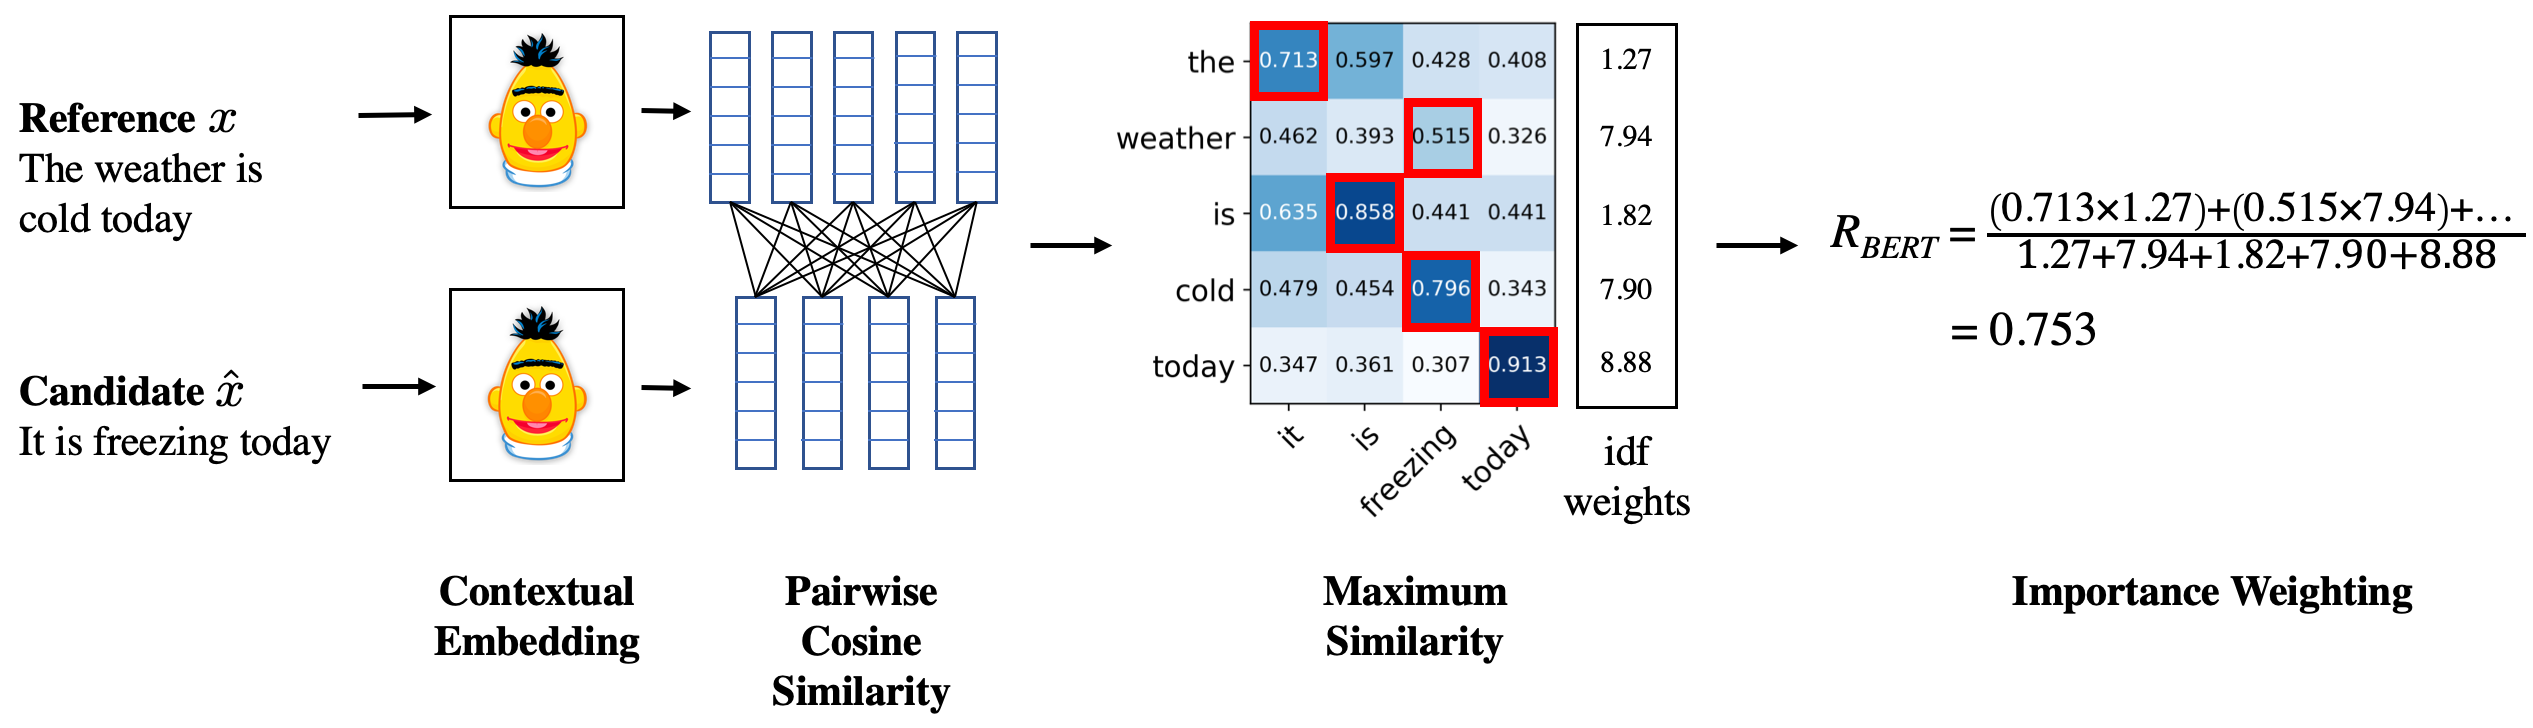
\includegraphics[width=\textwidth]{bert_score.png}
		\end{figure}
	}
	\only<4>{
		\frametitle{Métricas Mais Populares}
		\begin{itemize}
			\item BERTScore
			\item MoverScore
			\item BARTScore
		\end{itemize}
	}
	\only<5-8>{
		\frametitle{Problemas desse tipo de métrica}
		\begin{itemize}[<+(5)->]
			\item Alto custo computacional.
			\item Dependência de bons modelos.
			\item Caixa preta.
		\end{itemize}
	}
	\only<9>{
		\begin{figure}
			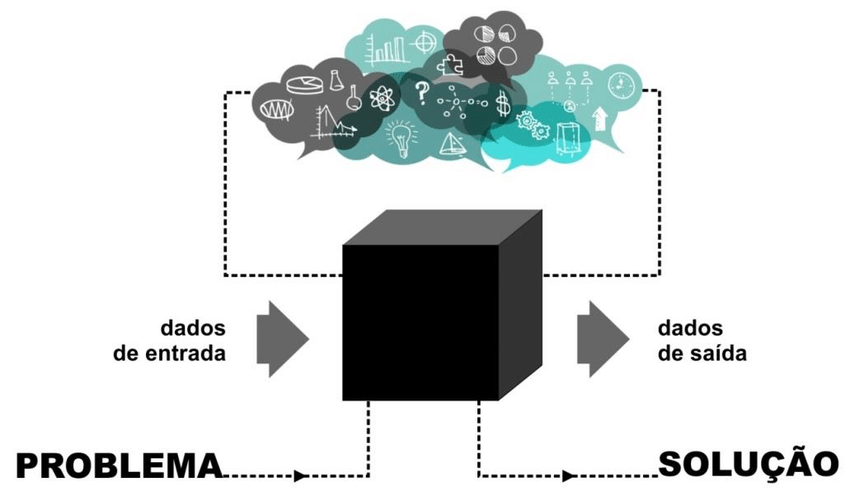
\includegraphics[width=0.9\textwidth]{Figura-31-Metodo-da-Caixa-Preta.png}
		\end{figure}
	}
\end{frame}

%----------------------------------------------------------------------------------------

\begin{frame}
	\frametitle{Problemática}
	\begin{itemize}[<+(1)->]
		\item Avaliar o desempenho de modelos é complexo.
		\item Novas métricas seguem surgindo.
		\item Qual métrica melhor se adequa a cada situação?
		\only<5>{
			\item Como as métricas se correlacionam com avaliação humana?
		}
		\only<6>{
			\item \textbf{Como as métricas se correlacionam com avaliação humana?}
		}
	\end{itemize}
\end{frame}

%----------------------------------------------------------------------------------------

\begin{frame}
	\frametitle{Objetivo}
	Mensurar a correlação entre diferentes métricas de avaliação automatizadas e 
	a forma de avaliação humana no âmbito de open-ended tasks.
\end{frame}
\section{Trabalhos Relacionados} % Seções são adicionadas para organizar sua apresentação em blocos discretos, todas as seções e subseções são automaticamente exibidas no índice como uma visão geral da apresentação, mas NÃO são exibidas como slides separados.

%----------------------------------------------------------------------------------------
\begin{frame}
    \frametitle{Timeline}
    \begin{figure}
        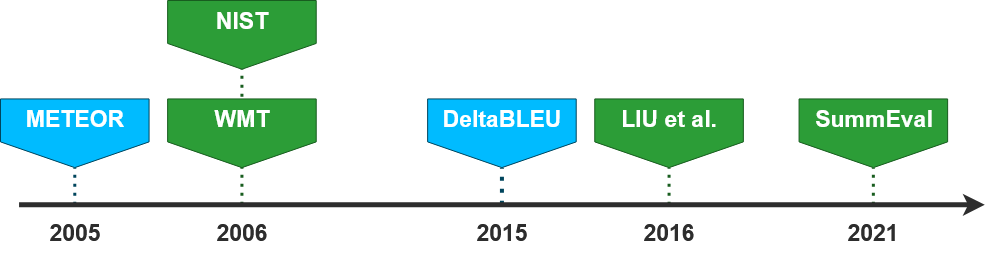
\includegraphics[width=0.9\textwidth]{TCC-timeline-trabalhos.png}
    \end{figure}
\end{frame}

%----------------------------------------------------------------------------------------
\begin{frame}
    \frametitle{SummEval}
    \only<1>{
        Um conjunto de recursos para pequisa de avaliação.
    }
    \only<2-3>{
        \begin{itemize}[<+(1)->]
            \item Sumários gerados no dataset CNN/DailyMail.
            \item Anotações humanas coletadas.
        \end{itemize}
    }
    \only<4->{
        \frametitle{Limitações do SummEval}
        \begin{itemize}[<+(4)->]
            \item Trabalha apenas com Sumarização.
            \item Focado somente na língua inglesa.
        \end{itemize}
    }
\end{frame}

%----------------------------------------------------------------------------------------
\begin{frame}
    \frametitle{Objetivo}
    \only<1>{
        Mensurar a correlação entre diferentes métricas de avaliação automatizadas e 
	    a forma de avaliação humana no âmbito de open-ended tasks.
    }
	\only<2>{
        Mensurar a correlação entre diferentes métricas de avaliação automatizadas e 
	    a forma de avaliação humana no âmbito de open-ended tasks \textbf{em português}.
    }
\end{frame}
% \section{Métricas} % Seções são adicionadas para organizar sua apresentação em blocos discretos, todas as seções e subseções são automaticamente exibidas no índice como uma visão geral da apresentação, mas NÃO são exibidas como slides separados.

%----------------------------------------------------------------------------------------

\begin{frame}
    \only<1-4>{
        \frametitle{ROUGE}
        \begin{itemize}[<+(1)->]
            \item Proposto por Lin et al. em 2004
            \item Faz uso de n-gramas
            \item É uma métrica baseada no Recall.
        \end{itemize}
    }
    \only<5>{
        \frametitle{ROUGE-N}
        \begin{equation} \tag{1}
            \label{eq:rouge-n-1}
            \text{Match}(\text{g}) =
            \min\left(\text{count}_{\text{ref}}(\text{g}), \text{count}_{\text{pred}}(\text{g}) \right)
        \end{equation}

        \begin{equation}
            \label{eq:rouge-n-2} \tag{2}
            \text{ROUGE-N} = 
            \frac{
            \sum_{\text{n-gram} \in ref}
            \text{Match}(\text{n-gram})
            }{
            \sum_{\text{n-gram} \in ref} \text{count}_{\text{ref}}(\text{n-gram})
            }
        \end{equation}
    }
    \only<6>{
        \frametitle{ROUGE-L}
        \begin{equation} \tag{1}
            \label{eq:rouge-l1} 
            R_{\text{LCS}} = \frac{ \text{LCS}(ref, pred) }{ ||ref|| }
            \quad\text{e}\quad
            P_{\text{LCS}} = \frac{ \text{LCS}(ref, pred) }{ ||pred|| }
        \end{equation}

        \begin{equation}
            \label{eq:rouge-l2} \tag{2}
            \text{ROUGE-L} =
            \frac{ 2 \cdot R_{\text{LCS}} \cdot P_{\text{LCS}} }
            { R_{\text{LCS}} + \cdot P_{\text{LCS}} }
        \end{equation}
    }
\end{frame}

%----------------------------------------------------------------------------------------

\begin{frame}
    \frametitle{BLEU}
    \only<1-6>{
        \begin{itemize}[<+(1)->]
            \item Proposto por Papineni et al. em 2002
            \item Focada em Tradução
            \item Faz uso de n-gramas
            \item É uma métrica baseada no Precisão
            \item Possui punição por brevidade
        \end{itemize}
    }
    \only<7>{
        \begin{equation} \tag{1}
            \label{eq:precisionBLEU-1}
            \text{Match}(\text{g}) =
            \min\left(\text{count}_{\text{pred}}(\text{g}), \text{count}_{\text{ref}}(\text{g}) \right)
        \end{equation}

        \begin{equation} \tag{2}
            \label{eq:precisionBLEU-2}
            P_n = \frac{
            \sum_{\text{n-gram} \in pred} \text{Match}(\text{n-gram})
            }{
            \sum_{\text{n-gram} \in pred} \text{count}_{pred}(\text{n-gram})
            }
        \end{equation}
    }
    \only<8>{
        \begin{equation} \tag{1}
            \label{eq:penalidadeBLEU}
            \text{BP} = 
            \begin{cases}
                1, & \text{se } ||pred|| > ||ref|| \\
                e^{1 - \frac{||ref||}{||pred||}}, & \text{se } ||pred|| \leq ||ref||
            \end{cases}
        \end{equation}

        \begin{equation} \tag{2}
            \label{eq:BLEUval}
            \text{BLEU} = \text{BP} \times \exp\left( \sum_{n=1}^N w_n \log P_n \right)
        \end{equation}

        \vspace{30px}

        $w_n$ = $\frac{1}{n}$
    }
    
\end{frame}

%----------------------------------------------------------------------------------------
\begin{frame}
    \frametitle{METEOR}
    \only<1-6>{
        \begin{itemize}[<+(1)->]
            \item Proposto por Banerjee et al. em 2005
            \item Focada em Tradução
            \item Faz uso de unigramas
            \item Aceita sinônimos e variações morfológicas simples
            \item Possui punição com base no ordenamento das palavras
        \end{itemize}
    }
    \only<7>{
        \begin{equation} \tag{1}
            \label{eq:METEORp}
            P = \frac{\text{\#1-grams}}{||pred||}, \quad R = \frac{\text{\#1-grams}}{||ref||} \quad e \quad F_{\alpha} = \frac{P \cdot R}{\alpha \cdot P + (1 - \alpha) \cdot R}
        \end{equation}

        \begin{equation} \tag{2}
            \label{eq:METEORpenalidade}
            \text{Penalidade} = \gamma \cdot \left(\frac{\text{\#chunks}}{\text{\#1-grams}}\right)^{\beta}
        \end{equation}

        \begin{equation} \tag{3}
            \label{eq:METEORval}
            \text{METEOR} = (1 - \text{Penalidade}) \cdot F_{\alpha}
        \end{equation}

        \vspace{30px}

        $\alpha$ = 0.90 \\
        $\beta$  = 3.00 \\ 
        $\gamma$ = 0.50
    }
\end{frame}

%----------------------------------------------------------------------------------------

\begin{frame}
    \frametitle{BERTScore}
    \only<1-5>{
        \begin{itemize}[<+(1)->]
            \item Proposto por Zhang et al. em 2019
            \item Faz uso de PLMs (Modelo BERT)
            \item Cria embeddings contextuais das palavras
            \item Calcula a distância de cosseno entre elas
        \end{itemize}
    }
    \only<6>{
        \begin{figure}
            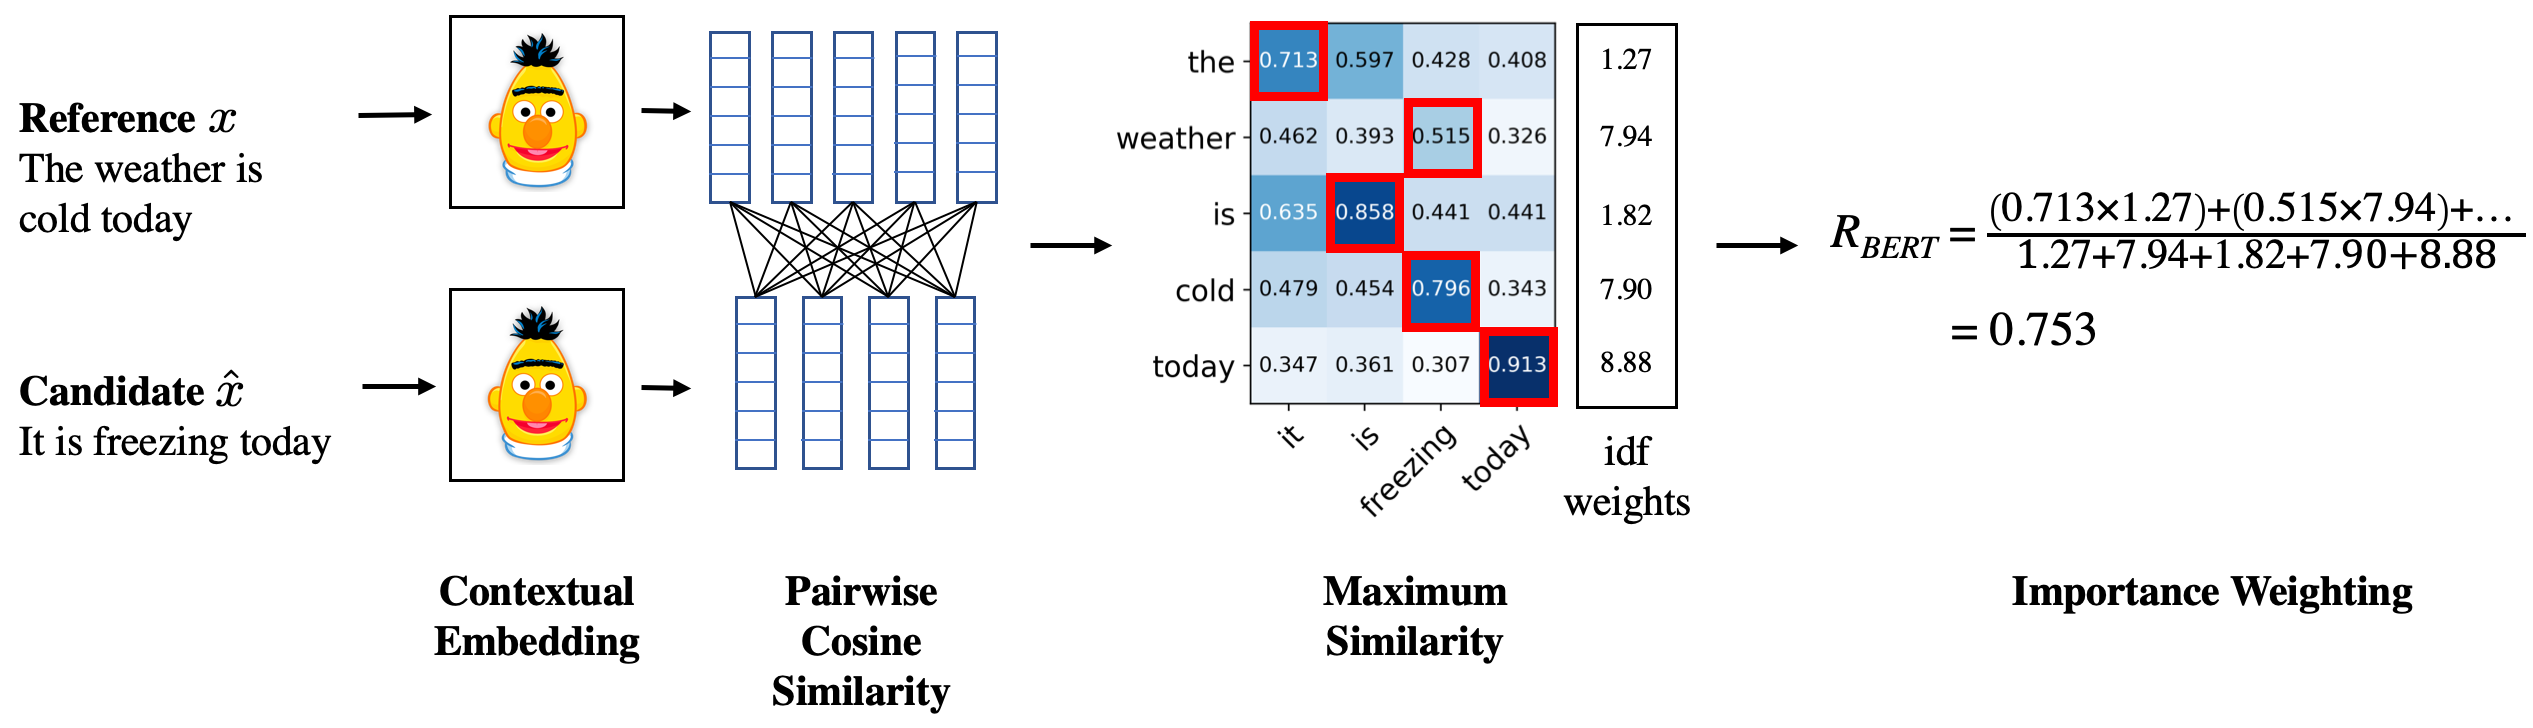
\includegraphics[width=\textwidth]{bert_score.png}
            % \caption{Fonte: \citet{bert-score}.}
        \end{figure}
    }
    \only<7>{
        \begin{equation} \tag{1}
            \label{eq:BERTScore-pr-1}
            P = \frac{1}{||pred||} \sum_{i=1}^{||pred||} \max_{j \in [1, ||ref||]} \text{Sim}(\text{pred}_i, \text{ref}_j)
        \end{equation}

        \begin{equation} \tag{2}
            \label{eq:BERTScore-pr2}
            R = \frac{1}{||ref||} \sum_{j=1}^{||ref||} \max_{i \in [1, ||pred||]} \text{Sim}(\text{ref}_j, \text{pred}_i)
        \end{equation}

        \begin{equation} \tag{3}
            \label{eq:BERTScore-f1}
            F_1 = \frac{2 \cdot P \cdot R}{P + R}
        \end{equation}
    }
\end{frame}

%----------------------------------------------------------------------------------------

\begin{frame}
    \frametitle{BARTScore}
    \only<1-4>{
        \begin{itemize}[<+(1)->]
            \item Proposto por Yuan et al. em 2021
            \item Faz uso de PLMs (Modelo BART)
            \item Calcula a probabilidade logaritmica de que o modelo BART gere a saída 
            dado um texto base
        \end{itemize}
    }
    \only<5->{
        \begin{equation} \tag{1}
            \label{eq:BARTScore-p}
            P = \text{Prob}_\text{Geração}(ref \rightarrow pred)
        \end{equation}

        \begin{equation} \tag{2}
            \label{eq:BARTScore-r}
            R = \text{Prob}_\text{Geração}(pred \rightarrow ref)
        \end{equation}

        \begin{equation} \tag{3}
            \label{eq:BARTScore-f1}
            F_1 = \frac{P + R}{2}
        \end{equation}
    }
\end{frame}

%----------------------------------------------------------------------------------------

\begin{frame}
    \frametitle{MoverScore}
    \only<1-7>{
        \begin{itemize}[<+(1)->]
            \item Proposto por Zhao et al. em 2019
            \item Faz uso de PLMs (Normalmente BERT)
            \item Realiza embedding contextial das palavras do texto
            \item Atribui às palavras um peso de importância baseado no TF-IDF
            \item Calcula o custo mínimo para alinhar os vetores
            \item Faz uso do Word Mover's Distance
        \end{itemize}
    }
    \only<8>{
        \begin{figure}
            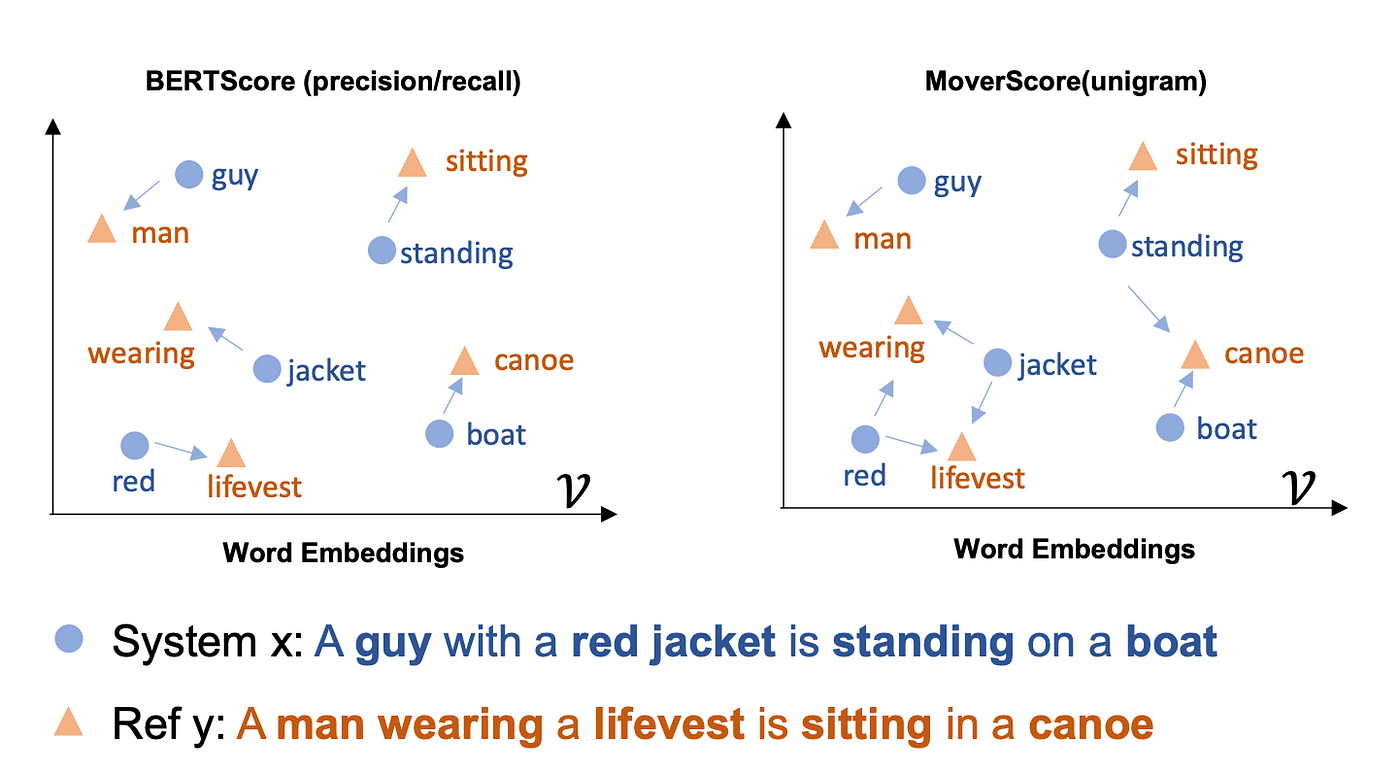
\includegraphics[width=0.8\textwidth]{moverscore.png}
            % \caption{Fonte: \citet{bert-score}.}
        \end{figure}
    }
\end{frame}
\section{Metodologia} % Seções são adicionadas para organizar sua apresentação em blocos discretos, todas as seções e subseções são automaticamente exibidas no índice como uma visão geral da apresentação, mas NÃO são exibidas como slides separados.

%----------------------------------------------------------------------------------------

\begin{frame}
    \frametitle{Pipeline}
    \begin{figure}[h]
        \centering
        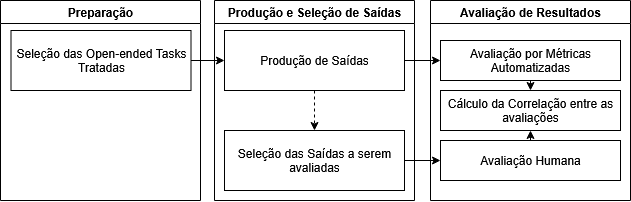
\includegraphics[width=0.95\textwidth]{TCC-Pipeline.png}
        \caption{Pipeline do Trabalho}
        \label{fig:Pipeline}
    \end{figure}
\end{frame}

%----------------------------------------------------------------------------------------

\begin{frame} 
    \only<1>{
        \begin{figure}[h]
            \centering
            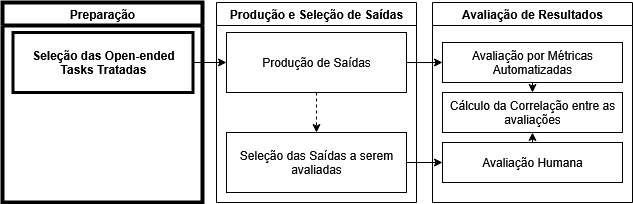
\includegraphics[width=0.95\textwidth]{TCC-Pipeline-tarefas.png}
            \caption{Etapa Atual: Seleção das Tarefas}
        \end{figure}
    }
    \only<2>{
        \frametitle{Tarefas Tratadas}
        \begin{columns}
            \column{0.5\linewidth}
                \begin{figure}
                    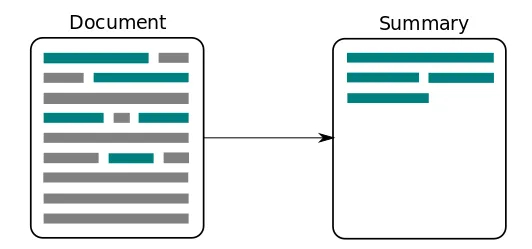
\includegraphics[width=0.8\textwidth]{summ.png}
                    \caption{Sumarização}
                \end{figure}
            \column{0.5\linewidth}
                \begin{figure}
                    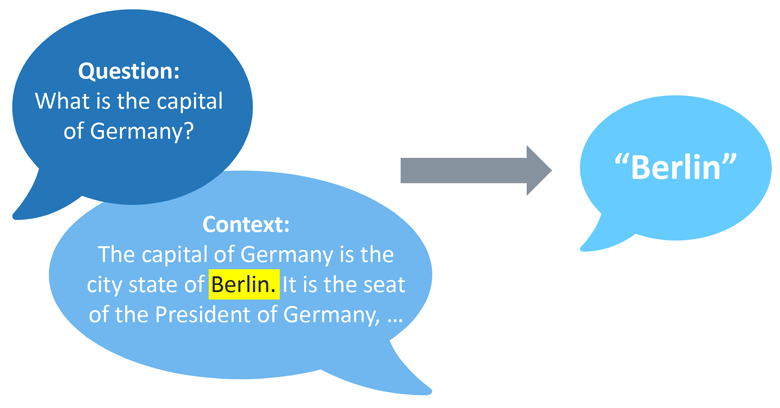
\includegraphics[width=0.8\textwidth]{qamainimage.png}
                    \caption{Question-Answering}
                \end{figure}
        \end{columns}
    }
    \only<3>{
		\frametitle{Abordagens Extrativas x Abstrativas}
		\begin{figure}
			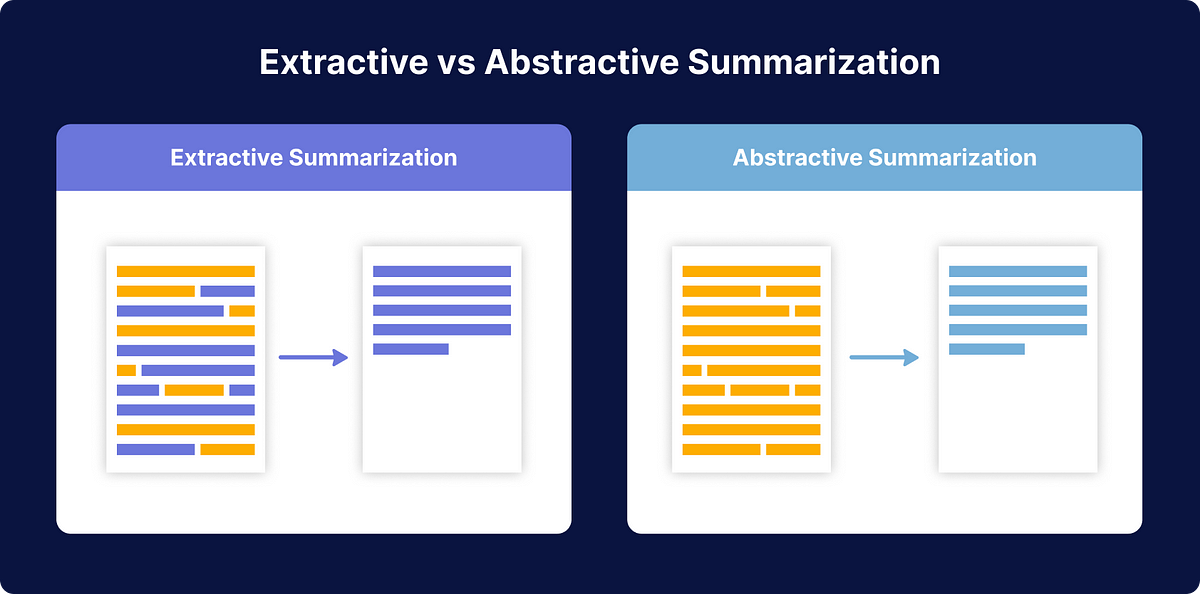
\includegraphics[width=0.8\textwidth]{abs_ext.png}
		\end{figure}
	}
\end{frame}

%----------------------------------------------------------------------------------------

\begin{frame}
    \only<1>{
        \begin{figure}[h]
            \centering
            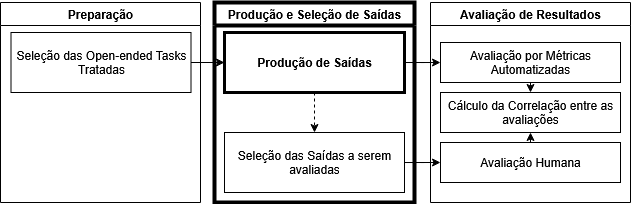
\includegraphics[width=0.95\textwidth]{TCC-Pipeline-producao.png}
            \caption{Etapa Atual: Produção das Saídas}
        \end{figure}
    }
    \only<2>{
        \frametitle{Modelos Utilizados}
        \begin{table}
            \centering
                \begin{tabular}{l c}
                    \hline
                    Tarefa & Modelo\\
                    \hline
                    Sumarização         & PTT5 Summ \\
                    Question-Answering  & Gemma 3   \\
                    \hline
                \end{tabular}
        \end{table}
    }
    \only<3-7>{
        \frametitle{Modelos Utilizados - Sumarização}

        Portuguese T5 for Abstractive Summarization (PTT5 Summ):
        \begin{itemize}[<+(3)->]
            \item Um PTT5 (Carmo et al., 2020) fine-tuned para sumarização
            \item Produzido por Paiola et al. em 2022
            \item Disponibilizado no HuggingFace por Recogna NLP
            \item O modelo escolhido foi fine-tuned sobre o dataset XL-Sum
        \end{itemize}
    }
    \only<8->{
        \frametitle{Modelos Utilizados - Question-Answering}

        Gemma 3:
        \begin{itemize}[<+(8)->]
            \item Uma família de modelos estado da arte leves
            \item Produzido pela Google em 2025
            \item Disponibilizado no HuggingFace pela Google
            \item A versão escolhida foi a it (Instruction Tuned) com 1B de parâmetros. 
        \end{itemize}
    }
\end{frame}

%----------------------------------------------------------------------------------------

\begin{frame}
    \only<1>{
        \frametitle{Datasets Utilizados}
        \begin{table}
            \centering
                \begin{tabular}{l c}
                    \hline
                    Tarefa & Dataset\\
                    \hline
                    Sumarização         & CNN Dailymail Azure Pt    \\
                    Question-Answering  & FairytaleQA Translated Pt \\
                    \hline
                \end{tabular}
        \end{table}
    }
    \only<2-5>{
        \frametitle{Datasets Utilizados - Sumarização}

        CNN Dailymail Azure Pt:
        \begin{itemize}[<+(2)->]
            \item Uma versão traduzida do CNN/DailyMail (Nallapati et al., 2016)
            \item Produzido por Rúben Almeida em 2023
            \item Disponibilizado no HuggingFace pelo autor
        \end{itemize}
    }
    \only<6-9>{
        \frametitle{Datasets Utilizados - Question-Answering}

        FairytaleQA Translated Pt:
        \begin{itemize}[<+(6)->]
            \item Uma versão traduzida do dataset FairyTaleQA (XU et al., 2022)
            \item Produzido por Leite et al. em 2024
            \item Disponibilizado no HuggingFace pelo autor
        \end{itemize}
    }
\end{frame}

%----------------------------------------------------------------------------------------

\begin{frame}
    \only<1>{
        \begin{figure}[h]
            \centering
            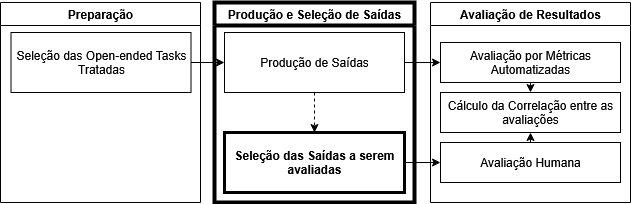
\includegraphics[width=0.95\textwidth]{TCC-Pipeline-selecao.png}
            \caption{Etapa Atual: Seleção das Saídas}
        \end{figure}
    }
    \only<2->{
        \frametitle{Seleção de Saídas}
        \begin{itemize}[<+(1)->]
            \item Amostragem aleatória
            \item 40 saídas por Tarefa
        \end{itemize}
    }
\end{frame}

%----------------------------------------------------------------------------------------

\begin{frame}
    \only<1>{
        \begin{figure}[h]
            \centering
            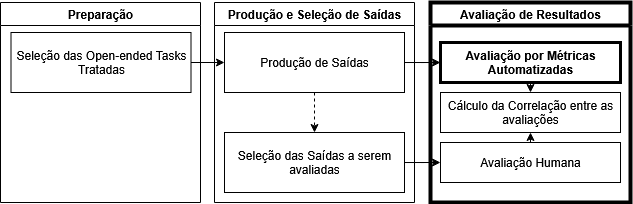
\includegraphics[width=0.95\textwidth]{TCC-Pipeline-metricas.png}
            \caption{Etapa Atual: Avaliação Automatizada}
        \end{figure}
    }
    \only<2>{
        \frametitle{Métricas}
        \begin{table}
            \centering
                \begin{tabular}{l c c c}
                    \hline
                    \textit{Métrica} & \textit{Baseada em} & \textit{Ano Criação} \\
                    \hline
                    \hline
                    BLEU       & $n$-gramas & 2002 \\
                    ROUGE      & $n$-gramas & 2004 \\
                    METEOR     & $n$-gramas & 2005 \\
                    BERTScore  & PLMs       & 2019 \\
                    MoverScore & PLMs       & 2019 \\
                    BARTScore  & PLMs       & 2021 \\
                    \hline
                \end{tabular}
            \caption{Descrição das métricas utilizadas}
        \end{table}
    }
\end{frame}

%----------------------------------------------------------------------------------------

\begin{frame}
    \only<1>{
        \begin{figure}[h]
            \centering
            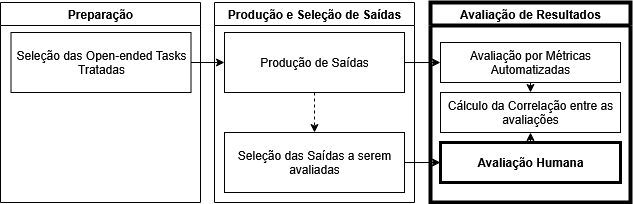
\includegraphics[width=0.95\textwidth]{TCC-Pipeline-humano.png}
            \caption{Etapa Atual: Avaliação Humana}
        \end{figure}
    }
    \only<2-6>{
        \frametitle{Avaliação Humana}
        \begin{itemize}[<+(1)->]
            \item Realizada com 8 pessoas
            \item Dividas em 2 grupos
            \item Cada grupo avaliou 20 saídas de cada tarefa
            \item Totalizando 80 saídas, avaliadas por 4 pessoas cada
            \item As avaliações são realizadas em \textbf{4 dimensões de qualidade}
        \end{itemize}
    }
    \only<7-12>{
        \frametitle{Dimensões de Qualidade}
        \only<7-11>{
            \begin{itemize}[<+(6)->]
                \item Coerência\only<7>{: Qualidade geral do texto}
                \item Consistência\only<8>{: Alinhamento entre a saída e o texto base}
                \item Fluência\only<9>{: Qualidade das frases geradas}
                \item Relevância\only<10>{: Pontos chave selecionados para o texto}
            \end{itemize}
        }
        \only<12>{
            \begin{itemize}
                \item Coerência
                \item Consistência
                \item \textbf{Naturalidade}
                \item Relevância
            \end{itemize}
        }
        
    }
    \only<13->{
        \frametitle{Avaliação Humana}
        \begin{itemize}
            \item Realizada com 8 pessoas
            \item Dividas em 2 grupos
            \item Cada grupo avaliou 20 saídas de cada tarefa
            \item Totalizando 80 saídas, avaliadas por 4 pessoas cada
            \item As avaliações são realizadas em 4 dimensões de qualidade
            \item \textbf{Valor final: a média das avaliações recebidas}
        \end{itemize}
    }
\end{frame}

%----------------------------------------------------------------------------------------

\begin{frame}
    \frametitle{Fomulários}
    \only<1-3>{
        \begin{enumerate}[<+(1)->]
            \item Seleciona seu grupo informado (1 ou 2).
            \item Lê os detalhes de cada saída.
        \end{enumerate}
    }
    \only<4>{
        \begin{table}
            \centering
            \begin{tabular}{l c c c}
                \hline
                \textit{Tarefa} & \textit{Saída} & \textit{Texto/Contexto Base} & \textit{Pergunta}\\
                \hline
                \hline
                Sumarização                 & \checkmark & \checkmark & $X$\\
                \textit{Question-Answering} & \checkmark & \checkmark & \checkmark\\
                \hline
            \end{tabular}
            \caption{Formatação do Formulário.}
            \label{tbl:forms}
        \end{table} 
    }
    \only<5>{
        \begin{enumerate}
            \item Seleciona seu grupo informado (1 ou 2).
            \item Lê os detalhes de cada saída.
            \item Avalia a saída.
        \end{enumerate}
    }
    \only<6>{
        Dimensões de Qualidade:
        \begin{itemize}
            \item Coerência
            \item Consistência
            \item Naturalidade
            \item Relevância
        \end{itemize}
    }
    \only<7>{
        \begin{columns}
            \column{0.5\linewidth}
            \begin{figure}
                
\includegraphics[width=0.8\textwidth]{forms-0.png}
                \caption{Escolha do Grupo}
            \end{figure}
            \begin{figure}
                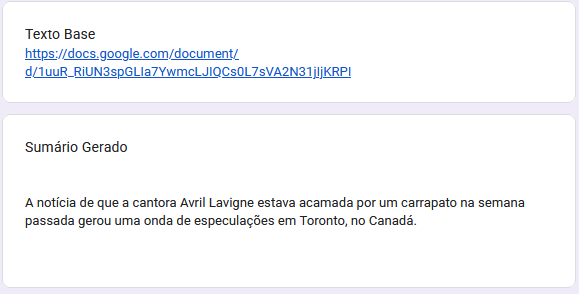
\includegraphics[width=0.8\textwidth]{forms-1.png}
                \caption{Descrição da Saída}
            \end{figure}
            \column{0.5\linewidth}
            \begin{figure}
                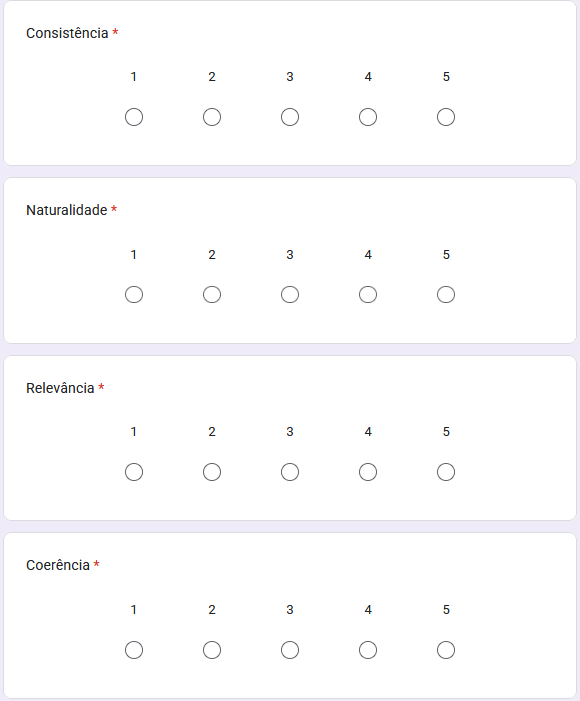
\includegraphics[width=0.8\textwidth]{forms-2.png}
                \caption{Campos de Avaliação}
            \end{figure}
        \end{columns}
    }
\end{frame}

%----------------------------------------------------------------------------------------

\begin{frame}
    \only<2-4>{
        \frametitle{Correlação de Pearson}
    }
    \only<1>{
        \begin{figure}[h]
            \centering
            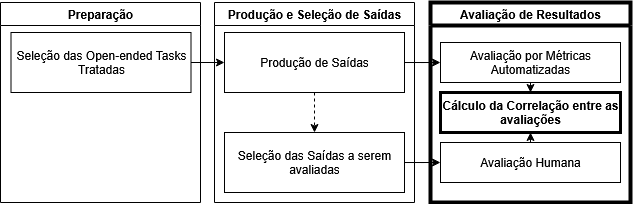
\includegraphics[width=0.95\textwidth]{TCC-Pipeline-correlacao.png}
            \caption{Etapa Atual: Cálculo da Correlação entre Avaliações}
        \end{figure}
    }
    \only<2-3>{
        \begin{itemize}[<+(1)->]
            \item Medida Estatística
            \item Quantificar as relações lineares entre duas variáveis
        \end{itemize}
    }
    \only<4>{
        \begin{table}[htbp]
            \centering
            \begin{tabular}{c l}
                \hline
                Valores de Pearson & Interpretação \\
                \hline
                0.90–1.00 & Muito forte    \\
                0.70–0.89 & Forte          \\
                0.40–0.69 & Moderada       \\
                0.10–0.39 & Fraca          \\
                0.00–0.10 & Negligenciável \\
                \hline
            \end{tabular}
            \caption{Discretização dos valores de Pearson.}
            \label{tbl:pearson}
        \end{table}
    }
    \only<5>{
        \frametitle{Pipeline}
        \begin{figure}[h]
            \centering
            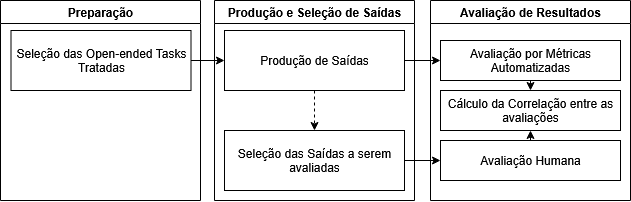
\includegraphics[width=0.95\textwidth]{TCC-Pipeline.png}
            \caption{Pipeline do Trabalho}
        \end{figure}
    }
\end{frame}
\section{Resultados} % Seções são adicionadas para organizar sua apresentação em blocos discretos, todas as seções e subseções são automaticamente exibidas no índice como uma visão geral da apresentação, mas NÃO são exibidas como slides separados.

%----------------------------------------------------------------------------------------

\begin{frame}
    \frametitle{Sumarização}
    \only<1>{
        \begin{table}[htbp]
            \centering
                \begin{tabular}{l c c}
                \hline
                Dimensão de Qualidade & Valor Médio & DP Médio\\
                \hline
                Consistência (AH) & 2.39 & 0.87\\
                Naturalidade (AH) & 3.58 & 0.97\\
                Relevância (AH)   & 2.46 & 0.97\\
                Coerência (AH)    & 2.59 & 0.95\\
                \hline
                \end{tabular}
            \caption{Médias de Avaliações Humanas para a tarefa de Sumarização.}
        \end{table}
    }
    \only<2>{
        \begin{table}
            \centering
            \resizebox{\textwidth}{!}{
                \begin{tabular}{l c c c c}
                    \hline
                    Métrica & Consistência & Naturalidade & Relevância & Coerência \\
                    \hline
                    \hline
                    ROUGE-1 & 0.21 & 0.29 & 0.29 & 0.24\\
                    ROUGE-2 & 0.18 & 0.27 & 0.23 & 0.24\\
                    ROUGE-L & 0.28 & 0.36 & 0.38 & 0.35\\
                    BLEU    & 0.28 & 0.35 & 0.33 & 0.35\\
                    BLEU-1  & 0.31 & 0.28 & 0.28 & 0.27\\
                    BLEU-2  & 0.27 & 0.27 & 0.25 & 0.27\\
                    METEOR  & 0.32 & 0.30 & 0.27 & 0.32\\
                    \hline
                    BERTScore-p  & 0.38 & 0.37 & 0.37 & 0.42\\
                    BERTScore-r  & 0.38 & \textbf{0.40} & 0.40 & 0.39\\
                    BERTScore-f1 & 0.40 & \textbf{0.40} & 0.40 & \textbf{0.43}\\
                    BARTScore    & \textbf{0.42} & 0.38 & \textbf{0.44} & 0.40\\
                    MoverScore   & 0.26 & 0.30 & 0.32 & 0.29\\
                    \hline
                \end{tabular}
            }
            \caption{Valores de Pearson da tarefa de Sumarização.}
        \end{table}
    }
    \only<3>{
        \begin{table}
            \centering
            \begin{tabular}{c l}
                \hline
                Valores de Pearson & Interpretação \\
                \hline
                0.90–1.00 & Muito forte    \\
                0.70–0.89 & Forte          \\
                0.40–0.69 & Moderada       \\
                0.10–0.39 & Fraca          \\
                0.00–0.10 & Negligenciável \\
                \hline
            \end{tabular}
            \caption{Discretização dos valores de Pearson.}
        \end{table}
    }
\end{frame}

%----------------------------------------------------------------------------------------

\begin{frame}
    \frametitle{Question-Answering}
    \only<1>{
        \begin{table}
            \centering
                \begin{tabular}{l c c}
                \hline
                Dimensão de Qualidade & Valor Médio & DP Médio\\
                \hline
                Consistência (AH) & 3.44 & 0.80\\
                Naturalidade (AH) & 4.05 & 0.73\\
                Relevância (AH)   & 3.48 & 0.71\\
                Coerência (AH)    & 3.55 & 0.74\\
                \hline
                \end{tabular}
            \caption{Médias de Avaliações Humanas para a tarefa de QA.}
        \end{table}
    }
    \only<2>{
        \begin{table}
            \centering
            \resizebox{\textwidth}{!}{
                \begin{tabular}{l c c c c}
                    \hline
                    Métrica & Consistência & Naturalidade & Relevância & Coerência \\
                    \hline
                    \hline
                    ROUGE-1 & 0.58 & 0.45 & 0.56 & 0.55\\
                    ROUGE-2 & 0.50 & 0.33 & 0.51 & 0.49\\
                    ROUGE-L & 0.56 & 0.44 & 0.55 & 0.54\\
                    BLEU    & 0.43 & 0.24 & 0.44 & 0.43\\
                    BLEU-1  & 0.51 & 0.37 & 0.50 & 0.49\\
                    BLEU-2  & 0.53 & 0.37 & 0.53 & 0.52\\
                    METEOR  & \textbf{0.61} & 0.49 & 0.59 & \textbf{0.59}\\
                    \hline
                    BERTScore-p  & 0.57 & 0.45 & 0.58 & 0.56\\
                    BERTScore-r  & 0.59 & \textbf{0.51} & 0.60 & 0.57\\
                    BERTScore-f1 & 0.60 & 0.50 & \textbf{0.61} & \textbf{0.59}\\
                    BARTScore    & 0.60 & 0.48 & 0.58 & \textbf{0.59}\\
                    MoverScore   & 0.44 & 0.26 & 0.44 & 0.42\\
                    \hline
                \end{tabular}
            }
            \caption{Valores de Pearson da tarefa de Question-Answering.}
        \end{table}
    }
    \only<3>{
        \begin{figure}
            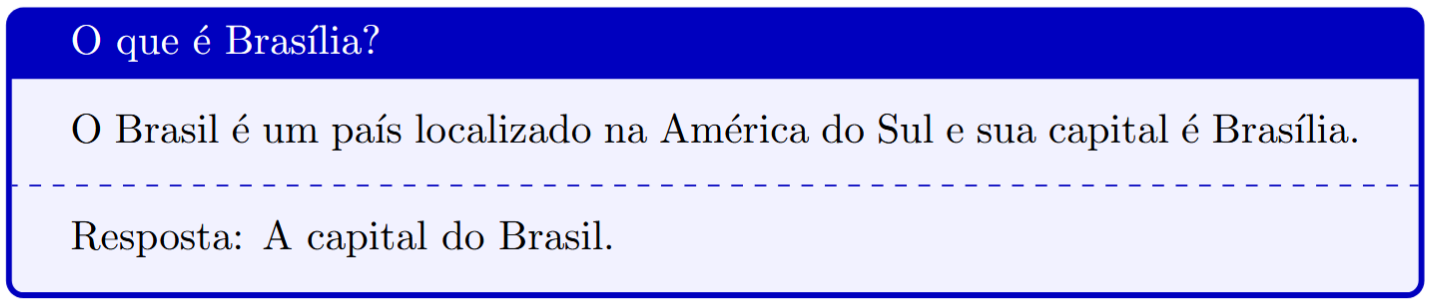
\includegraphics[width=0.9\textwidth]{QA.png}
        \end{figure}
    }
    \only<4>{
        \begin{figure}
            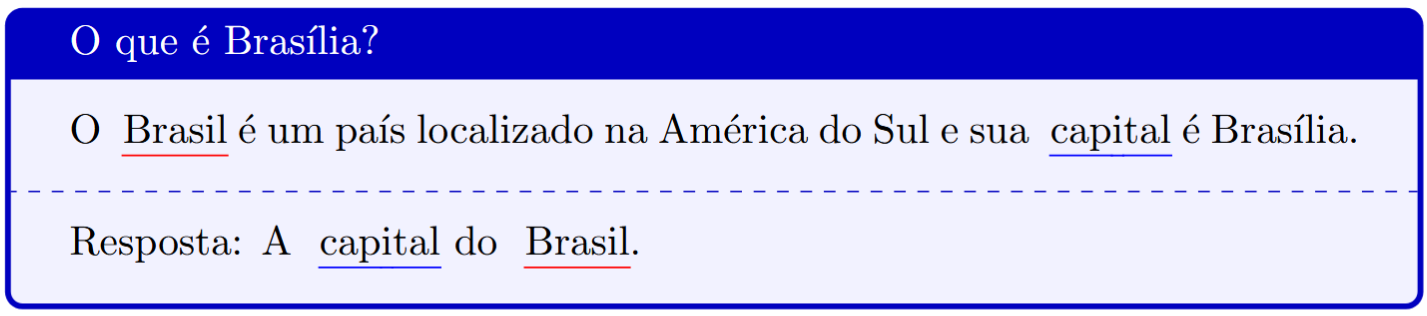
\includegraphics[width=0.9\textwidth]{qa-2.png}
        \end{figure}
    }
    \only<5>{
        \begin{table}
            \centering
            \resizebox{\textwidth}{!}{
                \begin{tabular}{l c c c c}
                    \hline
                    Métrica & Consistência & Naturalidade & Relevância & Coerência \\
                    \hline
                    \hline
                    ROUGE-1 & 0.58 & 0.45 & 0.56 & 0.55\\
                    ROUGE-2 & 0.50 & 0.33 & 0.51 & 0.49\\
                    ROUGE-L & 0.56 & 0.44 & 0.55 & 0.54\\
                    BLEU    & 0.43 & 0.24 & 0.44 & 0.43\\
                    BLEU-1  & 0.51 & 0.37 & 0.50 & 0.49\\
                    BLEU-2  & 0.53 & 0.37 & 0.53 & 0.52\\
                    METEOR  & \textbf{0.61} & 0.49 & 0.59 & \textbf{0.59}\\
                    \hline
                    BERTScore-p  & 0.57 & 0.45 & 0.58 & 0.56\\
                    BERTScore-r  & 0.59 & \textbf{0.51} & 0.60 & 0.57\\
                    BERTScore-f1 & 0.60 & 0.50 & \textbf{0.61} & \textbf{0.59}\\
                    BARTScore    & 0.60 & 0.48 & 0.58 & \textbf{0.59}\\
                    MoverScore   & 0.44 & 0.26 & 0.44 & 0.42\\
                    \hline
                \end{tabular}
            }
            \caption{Valores de Pearson da tarefa de Question-Answering.}
        \end{table}
    }
    \only<6>{
        \begin{table}[htbp]
            \centering
            \begin{tabular}{c l}
                \hline
                Valores de Pearson & Interpretação \\
                \hline
                0.90–1.00 & Muito forte    \\
                0.70–0.89 & Forte          \\
                0.40–0.69 & Moderada       \\
                0.10–0.39 & Fraca          \\
                0.00–0.10 & Negligenciável \\
                \hline
            \end{tabular}
            \caption{Discretização dos valores de Pearson.}
        \end{table}
    }
\end{frame}
\section{Conclusão} % Seções são adicionadas para organizar sua apresentação em blocos discretos, todas as seções e subseções são automaticamente exibidas no índice como uma visão geral da apresentação, mas NÃO são exibidas como slides separados.

%----------------------------------------------------------------------------------------
\begin{frame}
    \frametitle{Conclusão}
    \begin{itemize}[<+(1)->]
        \item Métricas baseadas em PLMs desempenharam melhor
        \item METEOR foi a melhor métrica baseada em N-gramas
        \item BERTScore e BARTScore tiveram os melhores resultados
        \item Correlação média/baixa
    \end{itemize}
\end{frame}

%----------------------------------------------------------------------------------------

\begin{frame}
    \frametitle{Limitações}
    \begin{itemize}
        \item Qualidade dos datasets.
        \item Qualidade dos modelos.
    \end{itemize}
\end{frame}

%----------------------------------------------------------------------------------------

\begin{frame}
    \frametitle{Trabalhos Futuros}
    \begin{itemize}[<+(1)->]
        \item Desenvolvimento de um dataset especializado.
        \item Treinamento/fine-tunning de um modelo sobre esse novo dataset.
        \item Testes com novas métricas.
        \item Treinamento/fine-tunning de novos modelos para uso nas métricas baseadas em PLMs.
        \item Análise com uma população maior.
        \item Análise com especialistas.
        \item Desenvolvimento de novas métricas.
    \end{itemize}
\end{frame}

% Referências
% \begin{frame}{Referências}
%     \nocite{*}
%     \printbibliography[heading=none]
% \end{frame}

% Slide final
\begin{frame}
    \begin{center}
        {\Huge Obrigado pela Atenção!}
    \end{center}
\end{frame}

\end{document}


